\documentclass[../main/NEMO_manual]{subfiles}

\begin{document}

\chapter{Observation and Model Comparison (OBS)}
\label{chap:OBS}

%\subsubsection*{Changes record}
%\begin{tabular}{l||l|m{0.65\linewidth}}
%    Release   & Author        & Modifications \\
%    {\em 4.0} & {\em D. J. Lea} & {\em \NEMO\ 4.0 updates}  \\
%    {\em 3.6} & {\em M. Martin, A. Ryan} & {\em Add averaging operator, standalone obs oper} \\
%    {\em 3.4} & {\em D. J. Lea, M. Martin, ...} & {\em Initial version}  \\
%    {\em --\texttt{"}--} & {\em ... K. Mogensen, A. Vidard, A. Weaver} & {\em ---\texttt{"}---}  \\
%\end{tabular}

\chaptertoc

\paragraph{Changes record} ~\\

{\footnotesize
  \begin{tabularx}{\textwidth}{l||X|X}
    Release & Author(s) & Modifications \\
    \hline
    {\em   4.0} & {\em ...} & {\em ...} \\
    {\em   3.6} & {\em ...} & {\em ...} \\
    {\em   3.4} & {\em ...} & {\em ...} \\
    {\em <=3.4} & {\em ...} & {\em ...}
  \end{tabularx}
}

\clearpage

The observation and model comparison code, the observation operator (OBS), reads in observation files
(profile temperature and salinity, sea surface temperature, sea level anomaly, sea ice concentration, and velocity) and calculates an interpolated model equivalent value at the observation location and nearest model time step.
The resulting data are saved in a ``feedback'' file (or files).
The code was originally developed for use with the NEMOVAR data assimilation code,
but can be used for validation or verification of the model or with any other data assimilation system.

The OBS code is called from \mdl{nemogcm} for model initialisation and to calculate the model equivalent values for observations on the 0th time step.
The code is then called again after each time step from \mdl{step}.
The code is only activated if the \nam{obs}{obs} namelist logical \np{ln_diaobs}{ln\_diaobs} is set to true.

For all data types a 2D horizontal interpolator or averager is needed to
interpolate/average the model fields to the observation location.
For {\em in situ} profiles, a 1D vertical interpolator is needed in addition to
provide model fields at the observation depths.
This now works in a generalised vertical coordinate system.

Some profile observation types (\eg\ tropical moored buoys) are made available as daily averaged quantities.
The observation operator code can be set-up to calculate the equivalent daily average model temperature fields using
the \np{nn_profdavtypes}{nn\_profdavtypes} namelist array.
Some SST observations are equivalent to a night-time average value and
the observation operator code can calculate equivalent night-time average model SST fields by
setting the namelist value \np{ln_sstnight}{ln\_sstnight} to true.
Otherwise (by default) the model value from the nearest time step to the observation time is used.

The code is controlled by the namelist \nam{obs}{obs}.
See the following sections for more details on setting up the namelist.

In \autoref{sec:OBS_example} a test example of the observation operator code is introduced, including
where to obtain data and how to setup the namelist.
In \autoref{sec:OBS_details} some more technical details of the different observation types used are introduced, and we
also show a more complete namelist.
In \autoref{sec:OBS_theory} some of the theoretical aspects of the observation operator are described including
interpolation methods and running on multiple processors.
In \autoref{sec:OBS_sao} the standalone observation operator code is described.
In \autoref{sec:OBS_obsutils} we describe some utilities to help work with the files produced by the OBS code.

%% =================================================================================================
\section{Running the observation operator code example}
\label{sec:OBS_example}

In this section an example of running the observation operator code is described using
profile observation data which can be freely downloaded.
It shows how to adapt an existing run and build of \NEMO\ to run the observation operator. Note also the observation operator and the assimilation increments code are run in the ORCA2\_ICE\_OBS SETTE test.

\begin{enumerate}
\item Compile \NEMO.

\item Download some EN4 data from \href{http://www.metoffice.gov.uk/hadobs}{www.metoffice.gov.uk/hadobs}.
  Choose observations which are valid for the period of your test run because
  the observation operator compares the model and observations for a matching date and time.

\item Compile the OBSTOOLS code in the \path{tools} directory using:
\begin{cmds}
./maketools -n OBSTOOLS -m [ARCH]
\end{cmds}

replacing \texttt{[ARCH]} with the build architecture file for your machine. Note the tools are checked out from a separate location of the repository (under \path{/utils/tools}).

\item Convert the EN4 data into feedback format:
\begin{cmds}
enact2fb.exe profiles_01.nc EN.4.1.1.f.profiles.g10.YYYYMM.nc
\end{cmds}

\item Include the following in the \NEMO\ namelist to run the observation operator on this data:
\end{enumerate}

Options are defined through the \nam{obs}{obs} namelist variables.
The options \np{ln_t3d}{ln\_t3d} and \np{ln_s3d}{ln\_s3d} switch on the temperature and salinity profile observation operator code.
The filename or array of filenames are specified using the \np{cn_profbfiles}{cn\_profbfiles} variable.
The model grid points for a particular observation latitude and longitude are found using
the grid searching part of the code.
This can be expensive, particularly for large numbers of observations,
setting \np{ln_grid_search_lookup}{ln\_grid\_search\_lookup} allows the use of a lookup table which
is saved into an \np{cn_gridsearch}{cn\_gridsearch} file (or files).
This will need to be generated the first time if it does not exist in the run directory.
However, once produced it will significantly speed up future grid searches.
Setting \np{ln_grid_global}{ln\_grid\_global} means that the code distributes the observations evenly between processors.
Alternatively each processor will work with observations located within the model subdomain
(see \autoref{subsec:OBS_parallel}).

A number of utilities are now provided to plot the feedback files, convert and recombine the files.
These are explained in more detail in \autoref{sec:OBS_obsutils}.
Utilities to convert other input data formats into the feedback format are also described in
\autoref{sec:OBS_obsutils}.

%% =================================================================================================
\section{Technical details (feedback type observation file headers)}
\label{sec:OBS_details}

Here we show a more complete example namelist \nam{obs}{obs} and also show the NetCDF headers of
the observation files that may be used with the observation operator.

\begin{listing}
  \nlst{namobs}
  \caption{\forcode{&namobs}}
  \label{lst:namobs}
\end{listing}

The observation operator code uses the feedback observation file format for all data types.
All the observation files must be in NetCDF format.
Some example headers (produced using \mbox{\textit{ncdump~-h}}) for profile data, sea level anomaly and
sea surface temperature are in the following subsections.

%% =================================================================================================
\subsection{Profile feedback file}

\begin{clines}
netcdf profiles_01 {
dimensions:
     N_OBS = 603 ;
     N_LEVELS = 150 ;
     N_VARS = 2 ;
     N_QCF = 2 ;
     N_ENTRIES = 1 ;
     N_EXTRA = 1 ;
     STRINGNAM = 8 ;
     STRINGGRID = 1 ;
     STRINGWMO = 8 ;
     STRINGTYP = 4 ;
     STRINGJULD = 14 ;
variables:
     char VARIABLES(N_VARS, STRINGNAM) ;
          VARIABLES:long_name = "List of variables in feedback files" ;
     char ENTRIES(N_ENTRIES, STRINGNAM) ;
          ENTRIES:long_name = "List of additional entries for each variable in feedback files" ;
     char EXTRA(N_EXTRA, STRINGNAM) ;
          EXTRA:long_name = "List of extra variables" ;
     char STATION_IDENTIFIER(N_OBS, STRINGWMO) ;
          STATION_IDENTIFIER:long_name = "Station identifier" ;
     char STATION_TYPE(N_OBS, STRINGTYP) ;
          STATION_TYPE:long_name = "Code instrument type" ;
     double LONGITUDE(N_OBS) ;
          LONGITUDE:long_name = "Longitude" ;
          LONGITUDE:units = "degrees_east" ;
          LONGITUDE:_Fillvalue = 99999.f ;
     double LATITUDE(N_OBS) ;
          LATITUDE:long_name = "Latitude" ;
          LATITUDE:units = "degrees_north" ;
          LATITUDE:_Fillvalue = 99999.f ;
     double DEPTH(N_OBS, N_LEVELS) ;
          DEPTH:long_name = "Depth" ;
          DEPTH:units = "metre" ;
          DEPTH:_Fillvalue = 99999.f ;
     int DEPTH_QC(N_OBS, N_LEVELS) ;
          DEPTH_QC:long_name = "Quality on depth" ;
          DEPTH_QC:Conventions = "q where q =[0,9]" ;
          DEPTH_QC:_Fillvalue = 0 ;
     int DEPTH_QC_FLAGS(N_OBS, N_LEVELS, N_QCF) ;
          DEPTH_QC_FLAGS:long_name = "Quality flags on depth" ;
          DEPTH_QC_FLAGS:Conventions = "NEMOVAR flag conventions" ;
     double JULD(N_OBS) ;
          JULD:long_name = "Julian day" ;
          JULD:units = "days since JULD_REFERENCE" ;
          JULD:Conventions = "relative julian days with decimal part (as parts of day)" ;
          JULD:_Fillvalue = 99999.f ;
     char JULD_REFERENCE(STRINGJULD) ;
          JULD_REFERENCE:long_name = "Date of reference for julian days" ;
          JULD_REFERENCE:Conventions = "YYYYMMDDHHMMSS" ;
     int OBSERVATION_QC(N_OBS) ;
          OBSERVATION_QC:long_name = "Quality on observation" ;
          OBSERVATION_QC:Conventions = "q where q =[0,9]" ;
          OBSERVATION_QC:_Fillvalue = 0 ;
     int OBSERVATION_QC_FLAGS(N_OBS, N_QCF) ;
          OBSERVATION_QC_FLAGS:long_name = "Quality flags on observation" ;
          OBSERVATION_QC_FLAGS:Conventions = "NEMOVAR flag conventions" ;
          OBSERVATION_QC_FLAGS:_Fillvalue = 0 ;
     int POSITION_QC(N_OBS) ;
          POSITION_QC:long_name = "Quality on position (latitude and longitude)" ;
          POSITION_QC:Conventions = "q where q =[0,9]" ;
          POSITION_QC:_Fillvalue = 0 ;
     int POSITION_QC_FLAGS(N_OBS, N_QCF) ;
          POSITION_QC_FLAGS:long_name = "Quality flags on position" ;
          POSITION_QC_FLAGS:Conventions = "NEMOVAR flag conventions" ;
          POSITION_QC_FLAGS:_Fillvalue = 0 ;
     int JULD_QC(N_OBS) ;
          JULD_QC:long_name = "Quality on date and time" ;
          JULD_QC:Conventions = "q where q =[0,9]" ;
          JULD_QC:_Fillvalue = 0 ;
     int JULD_QC_FLAGS(N_OBS, N_QCF) ;
          JULD_QC_FLAGS:long_name = "Quality flags on date and time" ;
          JULD_QC_FLAGS:Conventions = "NEMOVAR flag conventions" ;
          JULD_QC_FLAGS:_Fillvalue = 0 ;
     int ORIGINAL_FILE_INDEX(N_OBS) ;
          ORIGINAL_FILE_INDEX:long_name = "Index in original data file" ;
          ORIGINAL_FILE_INDEX:_Fillvalue = -99999 ;
     float POTM_OBS(N_OBS, N_LEVELS) ;
          POTM_OBS:long_name = "Potential temperature" ;
          POTM_OBS:units = "Degrees Celsius" ;
          POTM_OBS:_Fillvalue = 99999.f ;
     float POTM_Hx(N_OBS, N_LEVELS) ;
          POTM_Hx:long_name = "Model interpolated potential temperature" ;
          POTM_Hx:units = "Degrees Celsius" ;
          POTM_Hx:_Fillvalue = 99999.f ;
     int POTM_QC(N_OBS) ;
          POTM_QC:long_name = "Quality on potential temperature" ;
          POTM_QC:Conventions = "q where q =[0,9]" ;
          POTM_QC:_Fillvalue = 0 ;
     int POTM_QC_FLAGS(N_OBS, N_QCF) ;
          POTM_QC_FLAGS:long_name = "Quality flags on potential temperature" ;
          POTM_QC_FLAGS:Conventions = "NEMOVAR flag conventions" ;
          POTM_QC_FLAGS:_Fillvalue = 0 ;
     int POTM_LEVEL_QC(N_OBS, N_LEVELS) ;
          POTM_LEVEL_QC:long_name = "Quality for each level on potential temperature" ;
          POTM_LEVEL_QC:Conventions = "q where q =[0,9]" ;
          POTM_LEVEL_QC:_Fillvalue = 0 ;
     int POTM_LEVEL_QC_FLAGS(N_OBS, N_LEVELS, N_QCF) ;
          POTM_LEVEL_QC_FLAGS:long_name = "Quality flags for each level on potential temperature" ;
          POTM_LEVEL_QC_FLAGS:Conventions = "NEMOVAR flag conventions" ;
          POTM_LEVEL_QC_FLAGS:_Fillvalue = 0 ;
     int POTM_IOBSI(N_OBS) ;
          POTM_IOBSI:long_name = "ORCA grid search I coordinate" ;
     int POTM_IOBSJ(N_OBS) ;
          POTM_IOBSJ:long_name = "ORCA grid search J coordinate" ;
     int POTM_IOBSK(N_OBS, N_LEVELS) ;
          POTM_IOBSK:long_name = "ORCA grid search K coordinate" ;
     char POTM_GRID(STRINGGRID) ;
          POTM_GRID:long_name = "ORCA grid search grid (T,U,V)" ;
     float PSAL_OBS(N_OBS, N_LEVELS) ;
          PSAL_OBS:long_name = "Practical salinity" ;
          PSAL_OBS:units = "PSU" ;
          PSAL_OBS:_Fillvalue = 99999.f ;
     float PSAL_Hx(N_OBS, N_LEVELS) ;
          PSAL_Hx:long_name = "Model interpolated practical salinity" ;
          PSAL_Hx:units = "PSU" ;
          PSAL_Hx:_Fillvalue = 99999.f ;
     int PSAL_QC(N_OBS) ;
          PSAL_QC:long_name = "Quality on practical salinity" ;
          PSAL_QC:Conventions = "q where q =[0,9]" ;
          PSAL_QC:_Fillvalue = 0 ;
     int PSAL_QC_FLAGS(N_OBS, N_QCF) ;
          PSAL_QC_FLAGS:long_name = "Quality flags on practical salinity" ;
          PSAL_QC_FLAGS:Conventions = "NEMOVAR flag conventions" ;
          PSAL_QC_FLAGS:_Fillvalue = 0 ;
     int PSAL_LEVEL_QC(N_OBS, N_LEVELS) ;
          PSAL_LEVEL_QC:long_name = "Quality for each level on practical salinity" ;
          PSAL_LEVEL_QC:Conventions = "q where q =[0,9]" ;
          PSAL_LEVEL_QC:_Fillvalue = 0 ;
     int PSAL_LEVEL_QC_FLAGS(N_OBS, N_LEVELS, N_QCF) ;
          PSAL_LEVEL_QC_FLAGS:long_name = "Quality flags for each level on practical salinity" ;
          PSAL_LEVEL_QC_FLAGS:Conventions = "NEMOVAR flag conventions" ;
          PSAL_LEVEL_QC_FLAGS:_Fillvalue = 0 ;
     int PSAL_IOBSI(N_OBS) ;
          PSAL_IOBSI:long_name = "ORCA grid search I coordinate" ;
     int PSAL_IOBSJ(N_OBS) ;
          PSAL_IOBSJ:long_name = "ORCA grid search J coordinate" ;
     int PSAL_IOBSK(N_OBS, N_LEVELS) ;
          PSAL_IOBSK:long_name = "ORCA grid search K coordinate" ;
     char PSAL_GRID(STRINGGRID) ;
          PSAL_GRID:long_name = "ORCA grid search grid (T,U,V)" ;
     float TEMP(N_OBS, N_LEVELS) ;
          TEMP:long_name = "Insitu temperature" ;
          TEMP:units = "Degrees Celsius" ;
          TEMP:_Fillvalue = 99999.f ;

// global attributes:
          :title = "NEMO observation operator output" ;
          :Convention = "NEMO unified observation operator output" ;
}
\end{clines}

%% =================================================================================================
\subsection{Sea level anomaly feedback file}

\begin{clines}
netcdf sla_01 {
dimensions:
     N_OBS = 41301 ;
     N_LEVELS = 1 ;
     N_VARS = 1 ;
     N_QCF = 2 ;
     N_ENTRIES = 1 ;
     N_EXTRA = 1 ;
     STRINGNAM = 8 ;
     STRINGGRID = 1 ;
     STRINGWMO = 8 ;
     STRINGTYP = 4 ;
     STRINGJULD = 14 ;
variables:
     char VARIABLES(N_VARS, STRINGNAM) ;
          VARIABLES:long_name = "List of variables in feedback files" ;
     char ENTRIES(N_ENTRIES, STRINGNAM) ;
          ENTRIES:long_name = "List of additional entries for each variable in feedback files" ;
     char EXTRA(N_EXTRA, STRINGNAM) ;
          EXTRA:long_name = "List of extra variables" ;
     char STATION_IDENTIFIER(N_OBS, STRINGWMO) ;
          STATION_IDENTIFIER:long_name = "Station identifier" ;
     char STATION_TYPE(N_OBS, STRINGTYP) ;
          STATION_TYPE:long_name = "Code instrument type" ;
     double LONGITUDE(N_OBS) ;
          LONGITUDE:long_name = "Longitude" ;
          LONGITUDE:units = "degrees_east" ;
          LONGITUDE:_Fillvalue = 99999.f ;
     double LATITUDE(N_OBS) ;
          LATITUDE:long_name = "Latitude" ;
          LATITUDE:units = "degrees_north" ;
          LATITUDE:_Fillvalue = 99999.f ;
     double DEPTH(N_OBS, N_LEVELS) ;
          DEPTH:long_name = "Depth" ;
          DEPTH:units = "metre" ;
          DEPTH:_Fillvalue = 99999.f ;
     int DEPTH_QC(N_OBS, N_LEVELS) ;
          DEPTH_QC:long_name = "Quality on depth" ;
          DEPTH_QC:Conventions = "q where q =[0,9]" ;
          DEPTH_QC:_Fillvalue = 0 ;
     int DEPTH_QC_FLAGS(N_OBS, N_LEVELS, N_QCF) ;
          DEPTH_QC_FLAGS:long_name = "Quality flags on depth" ;
          DEPTH_QC_FLAGS:Conventions = "NEMOVAR flag conventions" ;
     double JULD(N_OBS) ;
          JULD:long_name = "Julian day" ;
          JULD:units = "days since JULD_REFERENCE" ;
          JULD:Conventions = "relative julian days with decimal part (as parts of day)" ;
          JULD:_Fillvalue = 99999.f ;
     char JULD_REFERENCE(STRINGJULD) ;
          JULD_REFERENCE:long_name = "Date of reference for julian days" ;
          JULD_REFERENCE:Conventions = "YYYYMMDDHHMMSS" ;
     int OBSERVATION_QC(N_OBS) ;
          OBSERVATION_QC:long_name = "Quality on observation" ;
          OBSERVATION_QC:Conventions = "q where q =[0,9]" ;
          OBSERVATION_QC:_Fillvalue = 0 ;
     int OBSERVATION_QC_FLAGS(N_OBS, N_QCF) ;
          OBSERVATION_QC_FLAGS:long_name = "Quality flags on observation" ;
          OBSERVATION_QC_FLAGS:Conventions = "NEMOVAR flag conventions" ;
          OBSERVATION_QC_FLAGS:_Fillvalue = 0 ;
     int POSITION_QC(N_OBS) ;
          POSITION_QC:long_name = "Quality on position (latitude and longitude)" ;
          POSITION_QC:Conventions = "q where q =[0,9]" ;
          POSITION_QC:_Fillvalue = 0 ;
     int POSITION_QC_FLAGS(N_OBS, N_QCF) ;
          POSITION_QC_FLAGS:long_name = "Quality flags on position" ;
          POSITION_QC_FLAGS:Conventions = "NEMOVAR flag conventions" ;
          POSITION_QC_FLAGS:_Fillvalue = 0 ;
     int JULD_QC(N_OBS) ;
          JULD_QC:long_name = "Quality on date and time" ;
          JULD_QC:Conventions = "q where q =[0,9]" ;
          JULD_QC:_Fillvalue = 0 ;
     int JULD_QC_FLAGS(N_OBS, N_QCF) ;
          JULD_QC_FLAGS:long_name = "Quality flags on date and time" ;
          JULD_QC_FLAGS:Conventions = "NEMOVAR flag conventions" ;
          JULD_QC_FLAGS:_Fillvalue = 0 ;
     int ORIGINAL_FILE_INDEX(N_OBS) ;
          ORIGINAL_FILE_INDEX:long_name = "Index in original data file" ;
          ORIGINAL_FILE_INDEX:_Fillvalue = -99999 ;
     float SLA_OBS(N_OBS, N_LEVELS) ;
          SLA_OBS:long_name = "Sea level anomaly" ;
          SLA_OBS:units = "metre" ;
          SLA_OBS:_Fillvalue = 99999.f ;
     float SLA_Hx(N_OBS, N_LEVELS) ;
          SLA_Hx:long_name = "Model interpolated sea level anomaly" ;
          SLA_Hx:units = "metre" ;
          SLA_Hx:_Fillvalue = 99999.f ;
     int SLA_QC(N_OBS) ;
          SLA_QC:long_name = "Quality on sea level anomaly" ;
          SLA_QC:Conventions = "q where q =[0,9]" ;
          SLA_QC:_Fillvalue = 0 ;
     int SLA_QC_FLAGS(N_OBS, N_QCF) ;
          SLA_QC_FLAGS:long_name = "Quality flags on sea level anomaly" ;
          SLA_QC_FLAGS:Conventions = "NEMOVAR flag conventions" ;
          SLA_QC_FLAGS:_Fillvalue = 0 ;
     int SLA_LEVEL_QC(N_OBS, N_LEVELS) ;
          SLA_LEVEL_QC:long_name = "Quality for each level on sea level anomaly" ;
          SLA_LEVEL_QC:Conventions = "q where q =[0,9]" ;
          SLA_LEVEL_QC:_Fillvalue = 0 ;
     int SLA_LEVEL_QC_FLAGS(N_OBS, N_LEVELS, N_QCF) ;
          SLA_LEVEL_QC_FLAGS:long_name = "Quality flags for each level on sea level anomaly" ;
          SLA_LEVEL_QC_FLAGS:Conventions = "NEMOVAR flag conventions" ;
          SLA_LEVEL_QC_FLAGS:_Fillvalue = 0 ;
     int SLA_IOBSI(N_OBS) ;
          SLA_IOBSI:long_name = "ORCA grid search I coordinate" ;
     int SLA_IOBSJ(N_OBS) ;
          SLA_IOBSJ:long_name = "ORCA grid search J coordinate" ;
     int SLA_IOBSK(N_OBS, N_LEVELS) ;
          SLA_IOBSK:long_name = "ORCA grid search K coordinate" ;
     char SLA_GRID(STRINGGRID) ;
          SLA_GRID:long_name = "ORCA grid search grid (T,U,V)" ;
     float MDT(N_OBS, N_LEVELS) ;
          MDT:long_name = "Mean Dynamic Topography" ;
          MDT:units = "metre" ;
          MDT:_Fillvalue = 99999.f ;

// global attributes:
          :title = "NEMO observation operator output" ;
          :Convention = "NEMO unified observation operator output" ;
}
\end{clines}

To use Sea Level Anomaly (SLA) data the mean dynamic topography (MDT) must be provided in a separate file defined on
the model grid called \textit{slaReferenceLevel.nc}.
The MDT is required in order to produce the model equivalent sea level anomaly from the model sea surface height.
Below is an example header for this file (on the ORCA025 grid).

\begin{clines}
dimensions:
        x = 1442 ;
        y = 1021 ;
variables:
        float nav_lon(y, x) ;
                nav_lon:units = "degrees_east" ;
        float nav_lat(y, x) ;
                nav_lat:units = "degrees_north" ;
        float sossheig(y, x) ;
                sossheig:_FillValue = -1.e+30f ;
                sossheig:coordinates = "nav_lon nav_lat" ;
                sossheig:long_name = "Mean Dynamic Topography" ;
                sossheig:units = "metres" ;
                sossheig:grid = "orca025T" ;
\end{clines}

%% =================================================================================================
\subsection{Sea surface temperature feedback file}

\begin{clines}
netcdf sst_01 {
dimensions:
     N_OBS = 33099 ;
     N_LEVELS = 1 ;
     N_VARS = 1 ;
     N_QCF = 2 ;
     N_ENTRIES = 1 ;
     STRINGNAM = 8 ;
     STRINGGRID = 1 ;
     STRINGWMO = 8 ;
     STRINGTYP = 4 ;
     STRINGJULD = 14 ;
variables:
     char VARIABLES(N_VARS, STRINGNAM) ;
          VARIABLES:long_name = "List of variables in feedback files" ;
     char ENTRIES(N_ENTRIES, STRINGNAM) ;
          ENTRIES:long_name = "List of additional entries for each variable in feedback files" ;
     char STATION_IDENTIFIER(N_OBS, STRINGWMO) ;
          STATION_IDENTIFIER:long_name = "Station identifier" ;
     char STATION_TYPE(N_OBS, STRINGTYP) ;
          STATION_TYPE:long_name = "Code instrument type" ;
     double LONGITUDE(N_OBS) ;
          LONGITUDE:long_name = "Longitude" ;
          LONGITUDE:units = "degrees_east" ;
          LONGITUDE:_Fillvalue = 99999.f ;
     double LATITUDE(N_OBS) ;
          LATITUDE:long_name = "Latitude" ;
          LATITUDE:units = "degrees_north" ;
          LATITUDE:_Fillvalue = 99999.f ;
     double DEPTH(N_OBS, N_LEVELS) ;
          DEPTH:long_name = "Depth" ;
          DEPTH:units = "metre" ;
          DEPTH:_Fillvalue = 99999.f ;
     int DEPTH_QC(N_OBS, N_LEVELS) ;
          DEPTH_QC:long_name = "Quality on depth" ;
          DEPTH_QC:Conventions = "q where q =[0,9]" ;
          DEPTH_QC:_Fillvalue = 0 ;
     int DEPTH_QC_FLAGS(N_OBS, N_LEVELS, N_QCF) ;
          DEPTH_QC_FLAGS:long_name = "Quality flags on depth" ;
          DEPTH_QC_FLAGS:Conventions = "NEMOVAR flag conventions" ;
     double JULD(N_OBS) ;
          JULD:long_name = "Julian day" ;
          JULD:units = "days since JULD_REFERENCE" ;
          JULD:Conventions = "relative julian days with decimal part (as parts of day)" ;
          JULD:_Fillvalue = 99999.f ;
     char JULD_REFERENCE(STRINGJULD) ;
          JULD_REFERENCE:long_name = "Date of reference for julian days" ;
          JULD_REFERENCE:Conventions = "YYYYMMDDHHMMSS" ;
     int OBSERVATION_QC(N_OBS) ;
          OBSERVATION_QC:long_name = "Quality on observation" ;
          OBSERVATION_QC:Conventions = "q where q =[0,9]" ;
          OBSERVATION_QC:_Fillvalue = 0 ;
     int OBSERVATION_QC_FLAGS(N_OBS, N_QCF) ;
          OBSERVATION_QC_FLAGS:long_name = "Quality flags on observation" ;
          OBSERVATION_QC_FLAGS:Conventions = "NEMOVAR flag conventions" ;
          OBSERVATION_QC_FLAGS:_Fillvalue = 0 ;
     int POSITION_QC(N_OBS) ;
          POSITION_QC:long_name = "Quality on position (latitude and longitude)" ;
          POSITION_QC:Conventions = "q where q =[0,9]" ;
          POSITION_QC:_Fillvalue = 0 ;
     int POSITION_QC_FLAGS(N_OBS, N_QCF) ;
          POSITION_QC_FLAGS:long_name = "Quality flags on position" ;
          POSITION_QC_FLAGS:Conventions = "NEMOVAR flag conventions" ;
          POSITION_QC_FLAGS:_Fillvalue = 0 ;
     int JULD_QC(N_OBS) ;
          JULD_QC:long_name = "Quality on date and time" ;
          JULD_QC:Conventions = "q where q =[0,9]" ;
          JULD_QC:_Fillvalue = 0 ;
     int JULD_QC_FLAGS(N_OBS, N_QCF) ;
          JULD_QC_FLAGS:long_name = "Quality flags on date and time" ;
          JULD_QC_FLAGS:Conventions = "NEMOVAR flag conventions" ;
          JULD_QC_FLAGS:_Fillvalue = 0 ;
     int ORIGINAL_FILE_INDEX(N_OBS) ;
          ORIGINAL_FILE_INDEX:long_name = "Index in original data file" ;
          ORIGINAL_FILE_INDEX:_Fillvalue = -99999 ;
     float SST_OBS(N_OBS, N_LEVELS) ;
          SST_OBS:long_name = "Sea surface temperature" ;
          SST_OBS:units = "Degree centigrade" ;
          SST_OBS:_Fillvalue = 99999.f ;
     float SST_Hx(N_OBS, N_LEVELS) ;
          SST_Hx:long_name = "Model interpolated sea surface temperature" ;
          SST_Hx:units = "Degree centigrade" ;
          SST_Hx:_Fillvalue = 99999.f ;
     int SST_QC(N_OBS) ;
          SST_QC:long_name = "Quality on sea surface temperature" ;
          SST_QC:Conventions = "q where q =[0,9]" ;
          SST_QC:_Fillvalue = 0 ;
     int SST_QC_FLAGS(N_OBS, N_QCF) ;
          SST_QC_FLAGS:long_name = "Quality flags on sea surface temperature" ;
          SST_QC_FLAGS:Conventions = "NEMOVAR flag conventions" ;
          SST_QC_FLAGS:_Fillvalue = 0 ;
     int SST_LEVEL_QC(N_OBS, N_LEVELS) ;
          SST_LEVEL_QC:long_name = "Quality for each level on sea surface temperature" ;
          SST_LEVEL_QC:Conventions = "q where q =[0,9]" ;
          SST_LEVEL_QC:_Fillvalue = 0 ;
     int SST_LEVEL_QC_FLAGS(N_OBS, N_LEVELS, N_QCF) ;
          SST_LEVEL_QC_FLAGS:long_name = "Quality flags for each level on sea surface temperature" ;
          SST_LEVEL_QC_FLAGS:Conventions = "NEMOVAR flag conventions" ;
          SST_LEVEL_QC_FLAGS:_Fillvalue = 0 ;
     int SST_IOBSI(N_OBS) ;
          SST_IOBSI:long_name = "ORCA grid search I coordinate" ;
     int SST_IOBSJ(N_OBS) ;
          SST_IOBSJ:long_name = "ORCA grid search J coordinate" ;
     int SST_IOBSK(N_OBS, N_LEVELS) ;
          SST_IOBSK:long_name = "ORCA grid search K coordinate" ;
     char SST_GRID(STRINGGRID) ;
          SST_GRID:long_name = "ORCA grid search grid (T,U,V)" ;

// global attributes:
          :title = "NEMO observation operator output" ;
          :Convention = "NEMO unified observation operator output" ;
}
\end{clines}

%% =================================================================================================
\section{Theoretical details}
\label{sec:OBS_theory}

%% =================================================================================================
\subsection{Horizontal interpolation and averaging methods}

For most observation types, the horizontal extent of the observation is small compared to the model grid size and so
the model equivalent of the observation is calculated by interpolating from
the four surrounding grid points to the observation location.
Some satellite observations (\eg\ microwave satellite SST data, or satellite SSS data) have a footprint which
is similar in size or larger than the model grid size (particularly when the grid size is small).
In those cases the model counterpart should be calculated by averaging the model grid points over
the same size as the footprint.
\NEMO\ therefore has the capability to specify either an interpolation or an averaging
(for surface observation types only).

The main namelist option associated with the interpolation/averaging is \np{nn_2dint}{nn\_2dint}.
This default option can be set to values from 0 to 6.
Values between 0 to 4 are associated with interpolation while values 5 or 6 are associated with averaging.
\begin{itemize}
\item \np[=0]{nn_2dint}{nn\_2dint}: Distance-weighted interpolation
\item \np[=1]{nn_2dint}{nn\_2dint}: Distance-weighted interpolation (small angle)
\item \np[=2]{nn_2dint}{nn\_2dint}: Bilinear interpolation (geographical grid)
\item \np[=3]{nn_2dint}{nn\_2dint}: Bilinear remapping interpolation (general grid)
\item \np[=4]{nn_2dint}{nn\_2dint}: Polynomial interpolation
\item \np[=5]{nn_2dint}{nn\_2dint}: Radial footprint averaging with diameter specified in the namelist as
  \texttt{rn\_[var]\_avglamscl} in degrees or metres (set using \texttt{ln\_[var]\_fp\_indegs})
\item \np[=6]{nn_2dint}{nn\_2dint}: Rectangular footprint averaging with E/W and N/S size specified in
  the namelist as \texttt{rn\_[var]\_avglamscl} and \texttt{rn\_[var]\_avgphiscl} in degrees or metres
  (set using \texttt{ln\_[var]\_fp\_indegs})
\end{itemize}
Replace \texttt{[var]} in the last two options with the observation type (sla, sst, sss or sic) for
which the averaging is to be performed (see namelist example above).
The \np{nn_2dint}{nn\_2dint} default option can be overridden for surface observation types using
namelist values \texttt{nn\_2dint\_[var]} where \texttt{[var]} is the observation type.

Below is some more detail on the various options for interpolation and averaging available in \NEMO.

%% =================================================================================================
\subsubsection{Horizontal interpolation}

Consider an observation point ${\mathrm P}$ with longitude and latitude (${\lambda_{}}_{\mathrm P}$, $\phi_{\mathrm P}$) and
the four nearest neighbouring model grid points ${\mathrm A}$, ${\mathrm B}$, ${\mathrm C}$ and ${\mathrm D}$ with
longitude and latitude ($\lambda_{\mathrm A}$, $\phi_{\mathrm A}$),($\lambda_{\mathrm B}$, $\phi_{\mathrm B}$) etc.
All horizontal interpolation methods implemented in \NEMO\ estimate the value of a model variable $x$ at point $P$ as
a weighted linear combination of the values of the model variables at the grid points ${\mathrm A}$, ${\mathrm B}$ etc.:

\begin{align*}
  {x_{}}_{\mathrm P} =
\frac{1}{w} \left( {w_{}}_{\mathrm A} {x_{}}_{\mathrm A} +
{w_{}}_{\mathrm B} {x_{}}_{\mathrm B} +
{w_{}}_{\mathrm C} {x_{}}_{\mathrm C} +
{w_{}}_{\mathrm D} {x_{}}_{\mathrm D} \right)
\end{align*}

where ${w_{}}_{\mathrm A}$, ${w_{}}_{\mathrm B}$ etc. are the respective weights for the model field at
points ${\mathrm A}$, ${\mathrm B}$ etc., and $w = {w_{}}_{\mathrm A} + {w_{}}_{\mathrm B} + {w_{}}_{\mathrm C} + {w_{}}_{\mathrm D}$.

Four different possibilities are available for computing the weights.

\begin{enumerate}
\item {\bfseries Great-Circle distance-weighted interpolation.}
  The weights are computed as a function of the great-circle distance $s(P, \cdot)$ between $P$ and
  the model grid points $A$, $B$ etc.
  For example, the weight given to the field ${x_{}}_{\mathrm A}$ is specified as the product of the distances
  from ${\mathrm P}$ to the other points:

  \begin{alignat*}{2}
    {w_{}}_{\mathrm A} = s({\mathrm P}, {\mathrm B}) \, s({\mathrm P}, {\mathrm C}) \, s({\mathrm P}, {\mathrm D})
  \end{alignat*}

  where

  \begin{alignat*}{2}
    s\left({\mathrm P}, {\mathrm M} \right) & = & \hspace{0.25em} \cos^{-1} \! \left\{
               \sin {\phi_{}}_{\mathrm P} \sin {\phi_{}}_{\mathrm M}
             + \cos {\phi_{}}_{\mathrm P} \cos {\phi_{}}_{\mathrm M}
               \cos ({\lambda_{}}_{\mathrm M} - {\lambda_{}}_{\mathrm P})
                   \right\}
   \end{alignat*}

   and $M$ corresponds to $B$, $C$ or $D$.
   A more stable form of the great-circle distance formula for small distances ($x$ near 1)
   involves the arcsine function (\eg\ see p.~101 of \citet{daley.barker_bk01}:

   \begin{alignat*}{2}
     s\left( {\mathrm P}, {\mathrm M} \right) = \sin^{-1} \! \left\{ \sqrt{ 1 - x^2 } \right\}
   \end{alignat*}

   where

   \begin{alignat*}{2}
     x = {a_{}}_{\mathrm M} {a_{}}_{\mathrm P} + {b_{}}_{\mathrm M} {b_{}}_{\mathrm P} + {c_{}}_{\mathrm M} {c_{}}_{\mathrm P}
   \end{alignat*}

   and

   \begin{alignat*}{3}
   & {a_{}}_{\mathrm M} & = && \quad \sin {\phi_{}}_{\mathrm M}, \\
   & {a_{}}_{\mathrm P} & = && \quad \sin {\phi_{}}_{\mathrm P}, \\
   & {b_{}}_{\mathrm M} & = && \quad \cos {\phi_{}}_{\mathrm M} \cos {\phi_{}}_{\mathrm M}, \\
   & {b_{}}_{\mathrm P} & = && \quad \cos {\phi_{}}_{\mathrm P} \cos {\phi_{}}_{\mathrm P}, \\
   & {c_{}}_{\mathrm M} & = && \quad \cos {\phi_{}}_{\mathrm M} \sin {\phi_{}}_{\mathrm M}, \\
   & {c_{}}_{\mathrm P} & = && \quad \cos {\phi_{}}_{\mathrm P} \sin {\phi_{}}_{\mathrm P}.
   \end{alignat*}

\item {\bfseries Great-Circle distance-weighted interpolation with small angle approximation.}
  Similar to the previous interpolation but with the distance $s$ computed as
  \begin{alignat*}{2}
    s\left( {\mathrm P}, {\mathrm M} \right)
    & = & \sqrt{ \left( {\phi_{}}_{\mathrm M} - {\phi_{}}_{\mathrm P} \right)^{2}
                                      + \left( {\lambda_{}}_{\mathrm M} - {\lambda_{}}_{\mathrm P} \right)^{2}
                                      \cos^{2} {\phi_{}}_{\mathrm M} }
  \end{alignat*}
  where $M$ corresponds to $A$, $B$, $C$ or $D$.

\item {\bfseries Bilinear interpolation for a regular spaced grid.}
  The interpolation is split into two 1D interpolations in the longitude and latitude directions, respectively.

\item {\bfseries Bilinear remapping interpolation for a general grid.}
  An iterative scheme that involves first mapping a quadrilateral cell into
  a cell with coordinates (0,0), (1,0), (0,1) and (1,1).
  This method is based on the \href{https://github.com/SCRIP-Project/SCRIP}{SCRIP interpolation package}.

\end{enumerate}

%% =================================================================================================
\subsubsection{Horizontal averaging}

For each surface observation type:
\begin{itemize}
\item The standard grid-searching code is used to find the nearest model grid point to the observation location
  (see next subsection).
\item The maximum number of grid points required for that observation in each local grid domain is calculated. Some of these points may later turn out to have zero weight depending on the shape of the footprint.
\item The longitudes and latitudes of the grid points surrounding the nearest model grid box are extracted using
  existing MPI routines.
\item The weights for each grid point associated with each observation are calculated,
  either for radial or rectangular footprints.
  For grid points completely within the footprint, the weight is one;
  for grid points completely outside the footprint, the weight is zero.
  For grid points which are partly within the footprint the ratio between the area of the footprint within
  the grid box and the total area of the grid box is used as the weight.
\item The weighted average of the model grid points associated with each observation is calculated,
  and this is then given as the model counterpart of the observation.
\end{itemize}

Examples of the weights calculated for an observation with rectangular and radial footprints are shown in
\autoref{fig:OBS_avgrec} and~\autoref{fig:OBS_avgrad}.

\begin{figure}
  \centering
  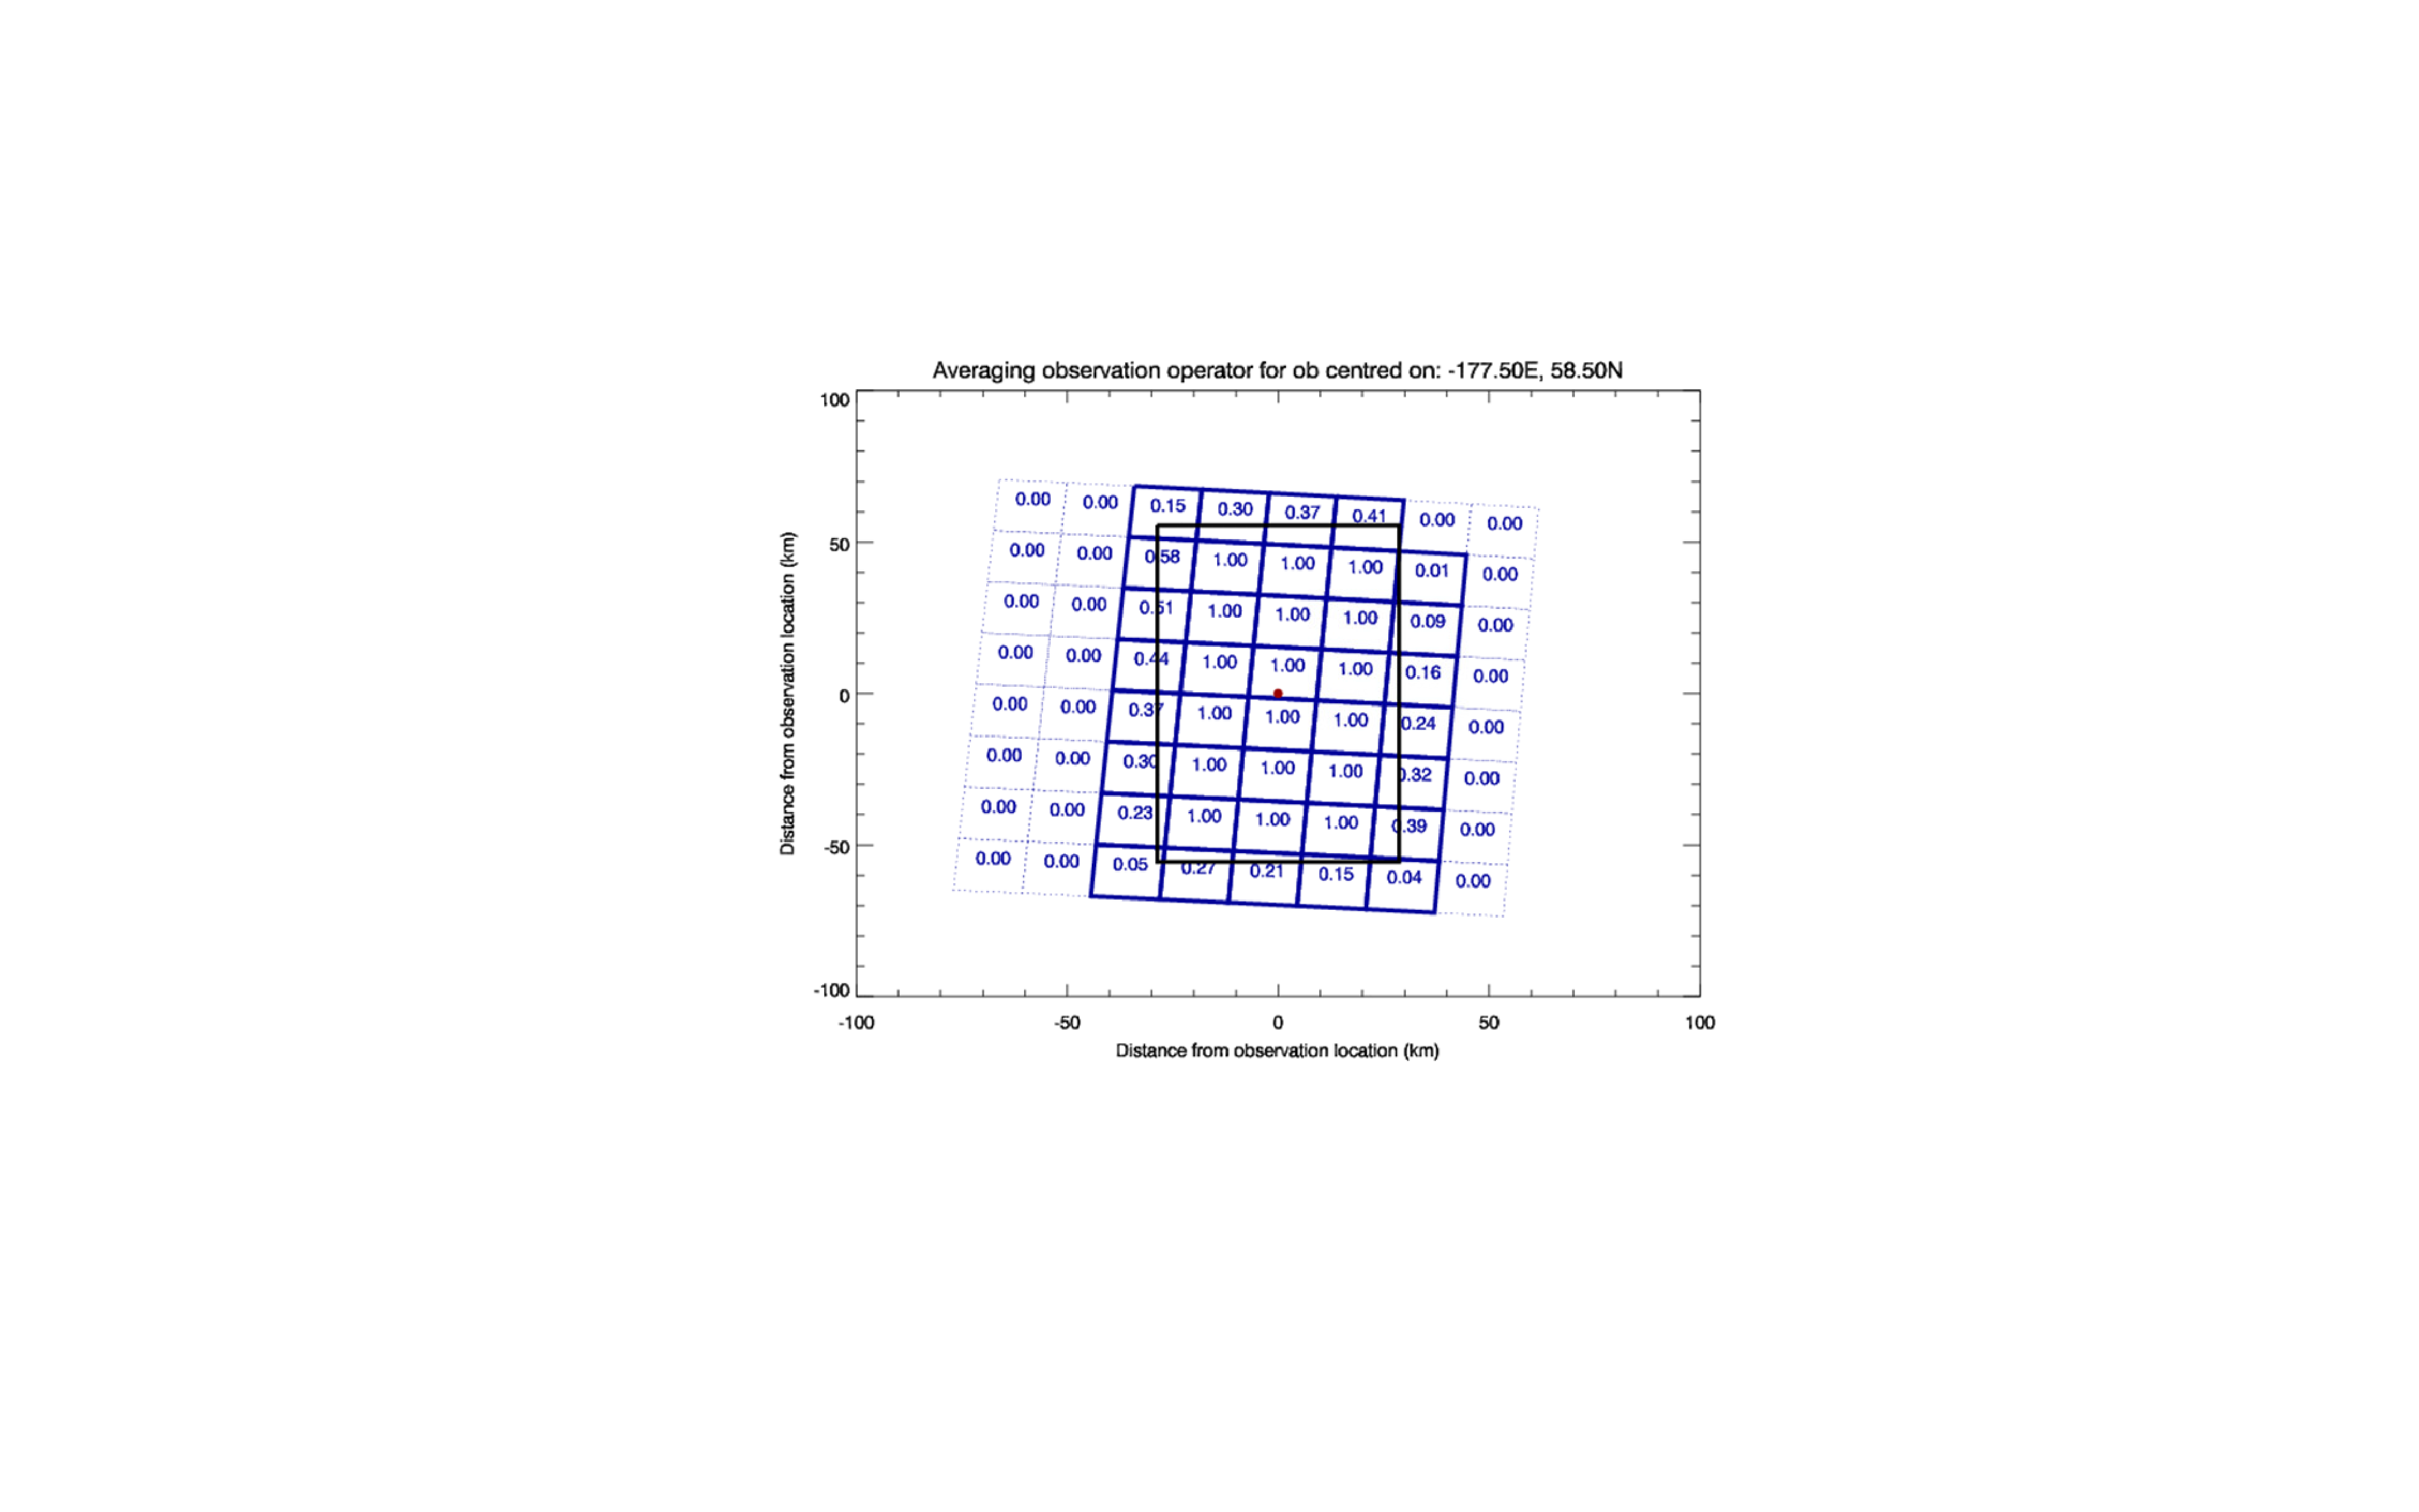
\includegraphics[width=0.66\textwidth]{OBS_avg_rec}
  \caption[Observational weights with a rectangular footprint]{
    Weights associated with each model grid box (blue lines and numbers)
    for an observation at -170.5\deg{E}, 56.0\deg{N} with a rectangular footprint of 1\deg\ x 1\deg.}
  \label{fig:OBS_avgrec}
\end{figure}

\begin{figure}
  \centering
  
\includegraphics[width=0.66\textwidth]{OBS_avg_rad}
  \caption[Observational weights with a radial footprint]{
    Weights associated with each model grid box (blue lines and numbers)
    for an observation at -170.5\deg{E}, 56.0\deg{N} with a radial footprint with diameter 1\deg.}
  \label{fig:OBS_avgrad}
\end{figure}

%% =================================================================================================
\subsection{Grid search}

For many grids used by the \NEMO\ model, such as the ORCA family, the horizontal grid coordinates $i$ and $j$ are not simple functions of latitude and longitude.
Therefore, it is not always straightforward to determine the grid points surrounding any given observational position.
Before the interpolation can be performed, a search algorithm is then required to determine the corner points of
the quadrilateral cell in which the observation is located.
This is the most difficult and time consuming part of the 2D interpolation procedure.
A robust test for determining if an observation falls within a given quadrilateral cell is as follows.
Let ${\mathrm P}({\lambda_{}}_{\mathrm P} ,{\phi_{}}_{\mathrm P} )$ denote the observation point,
and let ${\mathrm A}({\lambda_{}}_{\mathrm A} ,{\phi_{}}_{\mathrm A} )$, ${\mathrm B}({\lambda_{}}_{\mathrm B} ,{\phi_{}}_{\mathrm B} )$,
${\mathrm C}({\lambda_{}}_{\mathrm C} ,{\phi_{}}_{\mathrm C} )$ and ${\mathrm D}({\lambda_{}}_{\mathrm D} ,{\phi_{}}_{\mathrm D} )$
denote the bottom left, bottom right, top left and top right corner points of the cell, respectively.
To determine if P is inside the cell, we verify that the cross-products
\begin{align*}
  \begin{array}{lllll}
    {{\mathbf r}_{}}_{\mathrm PA} \times {{\mathbf r}_{}}_{\mathrm PC}
    & = & [({\lambda_{}}_{\mathrm A}\; -\; {\lambda_{}}_{\mathrm P} )
          ({\phi_{}}_{\mathrm C}   \; -\; {\phi_{}}_{\mathrm P} )
          - ({\lambda_{}}_{\mathrm C}\; -\; {\lambda_{}}_{\mathrm P} )
          ({\phi_{}}_{\mathrm A}   \; -\; {\phi_{}}_{\mathrm P} )] \; \widehat{\mathbf k} \\
    {{\mathbf r}_{}}_{\mathrm PB} \times {{\mathbf r}_{}}_{\mathrm PA}
    & = & [({\lambda_{}}_{\mathrm B}\; -\; {\lambda_{}}_{\mathrm P} )
          ({\phi_{}}_{\mathrm A}   \; -\; {\phi_{}}_{\mathrm P} )
          - ({\lambda_{}}_{\mathrm A}\; -\; {\lambda_{}}_{\mathrm P} )
          ({\phi_{}}_{\mathrm B}   \; -\; {\phi_{}}_{\mathrm P} )] \; \widehat{\mathbf k} \\
    {{\mathbf r}_{}}_{\mathrm PC} \times {{\mathbf r}_{}}_{\mathrm PD}
    & = & [({\lambda_{}}_{\mathrm C}\; -\; {\lambda_{}}_{\mathrm P} )
          ({\phi_{}}_{\mathrm D}   \; -\; {\phi_{}}_{\mathrm P} )
          - ({\lambda_{}}_{\mathrm D}\; -\; {\lambda_{}}_{\mathrm P} )
          ({\phi_{}}_{\mathrm C}   \; -\; {\phi_{}}_{\mathrm P} )] \; \widehat{\mathbf k} \\
    {{\mathbf r}_{}}_{\mathrm PD} \times {{\mathbf r}_{}}_{\mathrm PB}
    & = & [({\lambda_{}}_{\mathrm D}\; -\; {\lambda_{}}_{\mathrm P} )
          ({\phi_{}}_{\mathrm B}   \; -\; {\phi_{}}_{\mathrm P} )
          - ({\lambda_{}}_{\mathrm B}\; -\; {\lambda_{}}_{\mathrm P} )
          ({\phi_{}}_{\mathrm D}  \;  - \; {\phi_{}}_{\mathrm P} )] \; \widehat{\mathbf k} \\
  \end{array}
  % \label{eq:OBS_cross}
\end{align*}
point in the opposite direction to the unit normal $\widehat{\mathbf k}$
(\ie\ that the coefficients of $\widehat{\mathbf k}$ are negative),
where ${{\mathbf r}_{}}_{\mathrm PA}$, ${{\mathbf r}_{}}_{\mathrm PB}$, etc. correspond to
the vectors between points P and A, P and B, etc..
The method used is similar to the method used in the \href{https://github.com/SCRIP-Project/SCRIP}{SCRIP interpolation package}.

In order to speed up the grid search, there is the possibility to construct a lookup table for a user specified resolution.
This lookup table contains the lower and upper bounds on the $i$ and $j$ indices to
be searched for on a regular grid.
For each observation position, the closest point on the regular grid of this position is computed and
the $i$ and $j$ ranges of this point searched to determine the precise four points surrounding the observation.

%% =================================================================================================
\subsection{Parallel aspects of horizontal interpolation}
\label{subsec:OBS_parallel}

For horizontal interpolation, there is the basic problem that
the observations are unevenly distributed on the globe.
In \NEMO\ the model grid is divided into subgrids (or domains) where
each subgrid is executed on a single processing element with explicit message passing for
exchange of information along the domain boundaries when running on a massively parallel processor (MPP) system.

For observations there is no natural distribution since the observations are not equally distributed on the globe.
Two options have been made available:
1) geographical distribution;
and 2) round-robin.

%% =================================================================================================
\subsubsection{Geographical distribution of observations among processors}

\begin{figure}
  \centering
  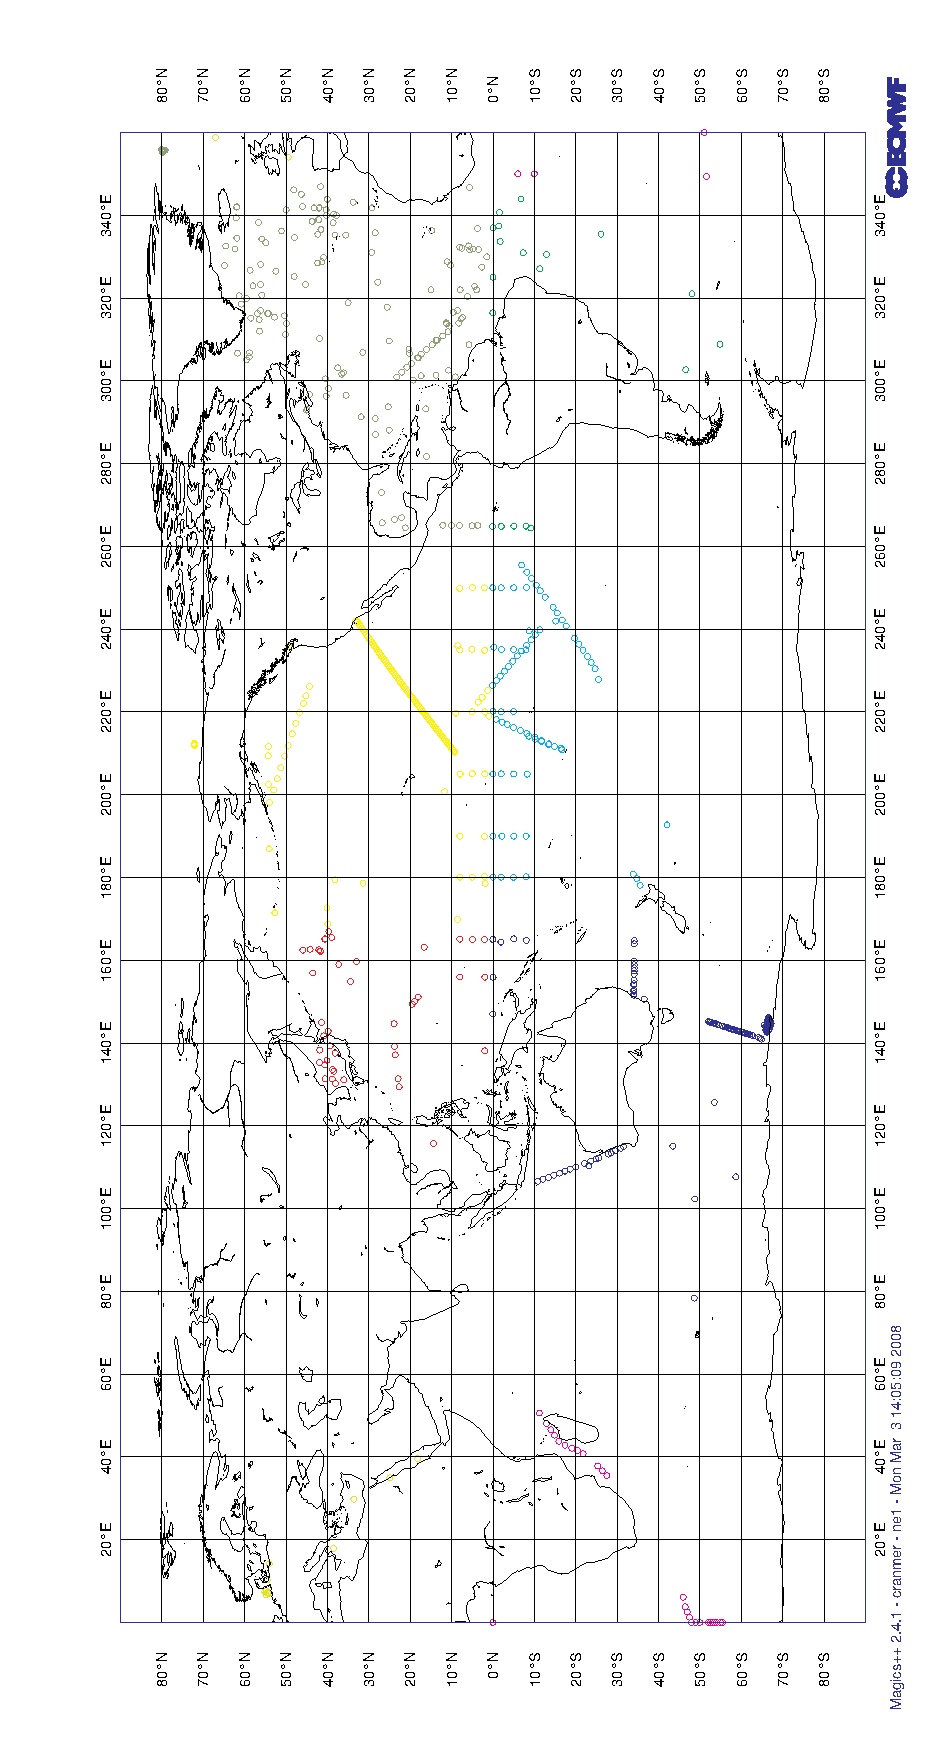
\includegraphics[width=0.66\textwidth]{OBS_obsdist_local}
  \caption[Observations with the geographical distribution]{
    Example of the distribution of observations with
    the geographical distribution of observational data}
  \label{fig:OBS_local}
\end{figure}

This is the simplest option in which the observations are distributed according to
the domain of the grid-point parallelization.
\autoref{fig:OBS_local} shows an example of the distribution of the {\em in situ} data on processors with
a different colour for each observation on a given processor for a 4 $\times$ 2 decomposition with ORCA2.
The grid-point domain decomposition is clearly visible on the plot.

The advantage of this approach is that all information needed for horizontal interpolation is available without
any MPP communication.
This is under the assumption that we are dealing with point observations and only using a $2 \times 2$ grid-point stencil for
the interpolation (\eg\ bilinear interpolation).
For higher order interpolation schemes this is no longer valid.
A disadvantage with the above scheme is that the number of observations on each processor can be very different.
If the cost of the actual interpolation is expensive relative to the communication of data needed for interpolation,
this could lead to load imbalance.

%% =================================================================================================
\subsubsection{Round-robin distribution of observations among processors}

\begin{figure}
  \centering
  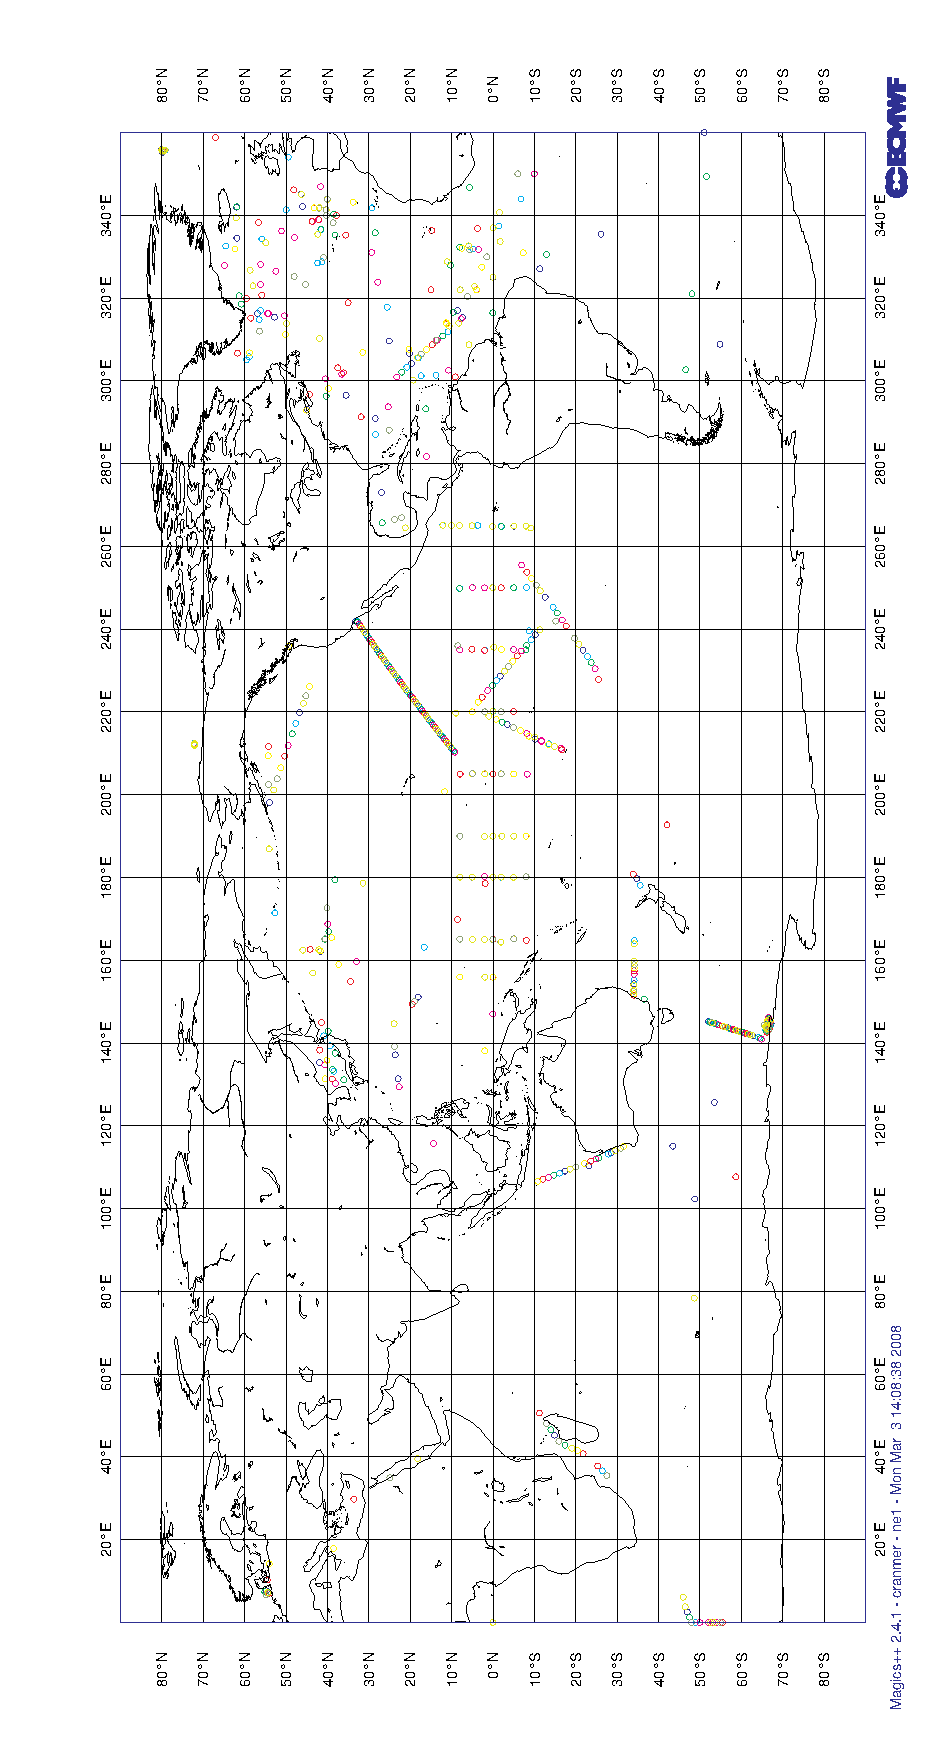
\includegraphics[width=0.66\textwidth]{OBS_obsdist_global}
  \caption[Observations with the round-robin distribution]{
    Example of the distribution of observations with
    the round-robin distribution of observational data.}
  \label{fig:OBS_global}
\end{figure}

An alternative approach is to distribute the observations equally among processors and
use message passing in order to retrieve the stencil for interpolation.
The simplest distribution of the observations is to distribute them using a round-robin scheme.
\autoref{fig:OBS_global} shows the distribution of the {\em in situ} data on processors for
the round-robin distribution of observations with a different colour for each observation on a given processor for
a 4 $\times$ 2 decomposition with ORCA2 for the same input data as in \autoref{fig:OBS_local}.
The observations are now clearly randomly distributed on the globe.
In order to be able to perform horizontal interpolation in this case,
a subroutine has been developed that retrieves any grid points in the global space.

%% =================================================================================================
\subsection{Vertical interpolation operator}

Vertical interpolation is achieved using either a cubic spline or linear interpolation.
For the cubic spline, the top and bottom boundary conditions for the second derivative of
the interpolating polynomial in the spline are set to zero.
At the bottom boundary, this is done using the land-ocean mask.

For profile observation types we do both vertical and horizontal interpolation. \NEMO\ has a generalised vertical coordinate system this means the vertical level depths can vary with location. Therefore, it is necessary first to perform vertical interpolation of the model value to the observation depths for each of the four surrounding grid points. After this the model values, at these points, at the observation depth, are horizontally interpolated to the observation location.

%\usepackage{framed}

%% =================================================================================================
\section{Standalone observation operator (\texttt{SAO})}
\label{sec:OBS_sao}

%% =================================================================================================
\subsection{Concept}

The observation operator maps model variables to observation space. This is normally done while the model is running, i.e. online, it is possible to apply this mapping offline without running the model with the \textbf{standalone observation operator} (SAO). The process is divided into an initialisation phase, an interpolation phase and an output phase.
During the interpolation phase the SAO populates the model arrays by
reading saved model fields from disk. The interpolation and the output phases use the same OBS code described in the preceding sections.

There are two ways of exploiting the standalone capacity.
The first is to mimic the behaviour of the online system by supplying model fields at
regular intervals between the start and the end of the run.
This approach results in a single model counterpart per observation.
This kind of usage produces feedback files the same file format as the online observation operator.
The second is to take advantage of the ability to run offline by calculating
multiple model counterparts for each observation.
In this case it is possible to consider all forecasts verifying at the same time.
By forecast, we mean any method which produces an estimate of physical reality which is not an observed value.

% sao.exe

%% =================================================================================================
\subsection{Using the standalone observation operator}

%% =================================================================================================
\subsubsection{Building}

In addition to \emph{OPA\_SRC} the SAO requires the inclusion of the \emph{SAO\_SRC} directory.
\emph{SAO\_SRC} contains a replacement \mdl{nemo} and \mdl{nemogcm} which
overwrites the resultant \textbf{nemo.exe}.
Note this a similar approach to that taken by the standalone surface scheme \emph{SAS\_SRC} and the offline TOP model \emph{OFF\_SRC}.

% Running
%% =================================================================================================
\subsubsection{Running}

The simplest way to use the executable is to edit and append the \nam{sao}{sao} namelist to
a full \NEMO\ namelist and then to run the executable as if it were nemo.exe.

% Configuration section
%% =================================================================================================
\subsection{Configuring the standalone observation operator}
The observation files and settings understood by \nam{obs}{obs} have been outlined in the online observation operator section.
In addition is a further namelist \nam{sao}{sao} which used to set the input model fields for the SAO

%% =================================================================================================
\subsubsection{Single field}

In the SAO the model arrays are populated at appropriate time steps via input files.
At present, \textbf{tsn} and \textbf{sshn} are populated by the default read routines.
These routines will be expanded upon in future versions to allow the specification of any model variable.
As such, input files must be global versions of the model domain with
\textbf{votemper}, \textbf{vosaline} and optionally \textbf{sshn} present.

For each field read there must be an entry in the \nam{sao}{sao} namelist specifying
the name of the file to read and the index along the \emph{time\_counter}.
For example, to read the second time counter from a single file the namelist would be.

\begin{listing}
  \begin{forlines}
!----------------------------------------------------------------------
!       namsao Standalone obs_oper namelist
!----------------------------------------------------------------------
!   sao_files    specifies the files containing the model counterpart
!   nn_sao_idx   specifies the time_counter index within the model file
&namsao
   sao_files = "foo.nc"
   nn_sao_idx = 2
/
  \end{forlines}
  \caption{\forcode{&namsao}}
  \label{lst:namsao}
\end{listing}

%% =================================================================================================
\subsubsection{Multiple fields per run}

Model field iteration is controlled via \textbf{nn\_sao\_freq} which
specifies the number of model steps at which the next field gets read.
For example, if 12 hourly fields are to be interpolated in a setup where 288 steps equals 24 hours.

\begin{forlines}
!----------------------------------------------------------------------
!       namsao Standalone obs_oper namelist
!----------------------------------------------------------------------
!   sao_files    specifies the files containing the model counterpart
!   nn_sao_idx   specifies the time_counter index within the model file
!   nn_sao_freq  specifies number of time steps between read operations
&namsao
   sao_files = "foo.nc" "foo.nc"
   nn_sao_idx = 1 2
   nn_sao_freq = 144
/
\end{forlines}

The above namelist will result in feedback files whose first 12 hours contain the first field of foo.nc and
the second 12 hours contain the second field.

%\begin{framed}
\textbf{Note} Missing files can be denoted as "nofile".
%\end{framed}

A collection of fields taken from a number of files at different indices can be combined at
a particular frequency in time to generate a pseudo model evolution.
If all that is needed is a single model counterpart at a regular interval then
the standard SAO is all that is required.
However, just to note, it is possible to extend this approach by comparing multiple forecasts, analyses, persisted analyses and
climatologies with the same set of observations.
This approach is referred to as \emph{Class 4} since it is the fourth metric defined by the GODAE intercomparison project. This requires multiple runs of the SAO and running an additional utility (not currently in the \NEMO\ repository) to combine the feedback files into one class 4 file.

%% =================================================================================================
\section{Observation utilities}
\label{sec:OBS_obsutils}

For convenience some tools for viewing and processing of observation and feedback files are provided in
the \NEMO\ repository.
These tools include OBSTOOLS which are a collection of \fortran\ programs which are helpful to deal with feedback files.
They do such tasks as observation file conversion, printing of file contents,
some basic statistical analysis of feedback files.
The other main tool is an IDL program called dataplot which uses a graphical interface to
visualise observations and feedback files.
OBSTOOLS and dataplot are described in more detail below.

%% =================================================================================================
\subsection{Obstools}

A series of \fortran\ utilities is provided with \NEMO\ called OBSTOOLS.
This are helpful in handling observation files and the feedback file output from the observation operator. A brief description of some of the utilities follows

%% =================================================================================================
\subsubsection{corio2fb}

The program corio2fb converts profile observation files from the Coriolis format to the standard feedback format.
It is called in the following way:

\begin{cmds}
corio2fb.exe outputfile inputfile1 inputfile2 ...
\end{cmds}

%% =================================================================================================
\subsubsection{enact2fb}

The program enact2fb converts profile observation files from the ENACT format to the standard feedback format.
It is called in the following way:

\begin{cmds}
enact2fb.exe outputfile inputfile1 inputfile2 ...
\end{cmds}

%% =================================================================================================
\subsubsection{fbcomb}

The program fbcomb combines multiple feedback files produced by individual processors in
an MPI run of \NEMO\ into a single feedback file.
It is called in the following way:

\begin{cmds}
fbcomb.exe outputfile inputfile1 inputfile2 ...
\end{cmds}

%% =================================================================================================
\subsubsection{fbmatchup}

The program fbmatchup will match observations from two feedback files.
It is called in the following way:

\begin{cmds}
fbmatchup.exe outputfile inputfile1 varname1 inputfile2 varname2 ...
\end{cmds}

%% =================================================================================================
\subsubsection{fbprint}

The program fbprint will print the contents of a feedback file or files to standard output.
Selected information can be output using optional arguments.
It is called in the following way:

\begin{cmds}
fbprint.exe [options] inputfile

options:
     -b            shorter output
     -q            Select observations based on QC flags
     -Q            Select observations based on QC flags
     -B            Select observations based on QC flags
     -u            unsorted
     -s ID         select station ID
     -t TYPE       select observation type
     -v NUM1-NUM2  select variable range to print by number
                      (default all)
     -a NUM1-NUM2  select additional variable range to print by number
                      (default all)
     -e NUM1-NUM2  select extra variable range to print by number
                      (default all)
     -d            output date range
     -D            print depths
     -z            use zipped files
\end{cmds}

%% =================================================================================================
\subsubsection{fbsel}

The program fbsel will select or subsample observations.
It is called in the following way:

\begin{cmds}
fbsel.exe <input filename> <output filename>
\end{cmds}

%% =================================================================================================
\subsubsection{fbstat}

The program fbstat will output summary statistics in different global areas into a number of files.
It is called in the following way:

\begin{cmds}
fbstat.exe [-nmlev] <filenames>
\end{cmds}

%% =================================================================================================
\subsubsection{fbthin}

The program fbthin will thin the data to 1 degree resolution.
The code could easily be modified to thin to a different resolution.
It is called in the following way:

\begin{cmds}
fbthin.exe inputfile outputfile
\end{cmds}

%% =================================================================================================
\subsubsection{sla2fb}

The program sla2fb will convert an AVISO SLA format file to feedback format.
It is called in the following way:

\begin{cmds}
sla2fb.exe [-s type] outputfile inputfile1 inputfile2 ...

Option:
     -s            Select altimeter data_source
\end{cmds}

%% =================================================================================================
\subsubsection{vel2fb}

The program vel2fb will convert TAO/PIRATA/RAMA currents files to feedback format.
It is called in the following way:

\begin{cmds}
vel2fb.exe outputfile inputfile1 inputfile2 ...
\end{cmds}

%% =================================================================================================
\subsection{Building the obstools}

To build the obstools use in the tools directory use ./maketools -n OBSTOOLS -m [ARCH].

%% =================================================================================================
\subsection{Dataplot}

An IDL program called dataplot is included which uses a graphical interface to
visualise observations and feedback files. Note a similar package has recently developed in python (also called dataplot) which does some of the same things that the IDL dataplot does. Please contact the authors of the this chapter if you are interested in this.

It is possible to zoom in, plot individual profiles and calculate some basic statistics.
To plot some data run IDL and then:

\begin{verbatim}
IDL> dataplot, "filename"
\end{verbatim}

To read multiple files into dataplot,
for example multiple feedback files from different processors or from different days,
the easiest method is to use the spawn command to generate a list of files which can then be passed to dataplot.

\begin{verbatim}
IDL> spawn, 'ls profb*.nc', files
IDL> dataplot, files
\end{verbatim}

\autoref{fig:OBS_dataplotmain} shows the main window which is launched when dataplot starts.
This is split into three parts.
At the top there is a menu bar which contains a variety of drop down menus.
Areas - zooms into prespecified regions;
plot - plots the data as a timeseries or a T-S diagram if appropriate;
Find - allows data to be searched;
Config - sets various configuration options.

The middle part is a plot of the geographical location of the observations.
This will plot the observation value, the model background value or observation minus background value depending on
the option selected in the radio button at the bottom of the window.
The plotting colour range can be changed by clicking on the colour bar.
The title of the plot gives some basic information about the date range and depth range shown,
the extreme values, and the mean and RMS values.
It is possible to zoom in using a drag-box.
You may also zoom in or out using the mouse wheel.

The bottom part of the window controls what is visible in the plot above.
There are two bars which select the level range plotted (for profile data).
The other bars below select the date range shown.
The bottom of the figure allows the option to plot the mean, root mean square, standard deviation or
mean square values.
As mentioned above you can choose to plot the observation value, the model background value or
observation minus background value.
The next group of radio buttons selects the map projection.
This can either be regular longitude latitude grid, or north or south polar stereographic.
The next group of radio buttons will plot bad observations, switch to salinity and
plot density for profile observations.
The rightmost group of buttons will print the plot window as a postscript, save it as png, or exit from dataplot.

\begin{figure}
  \centering
  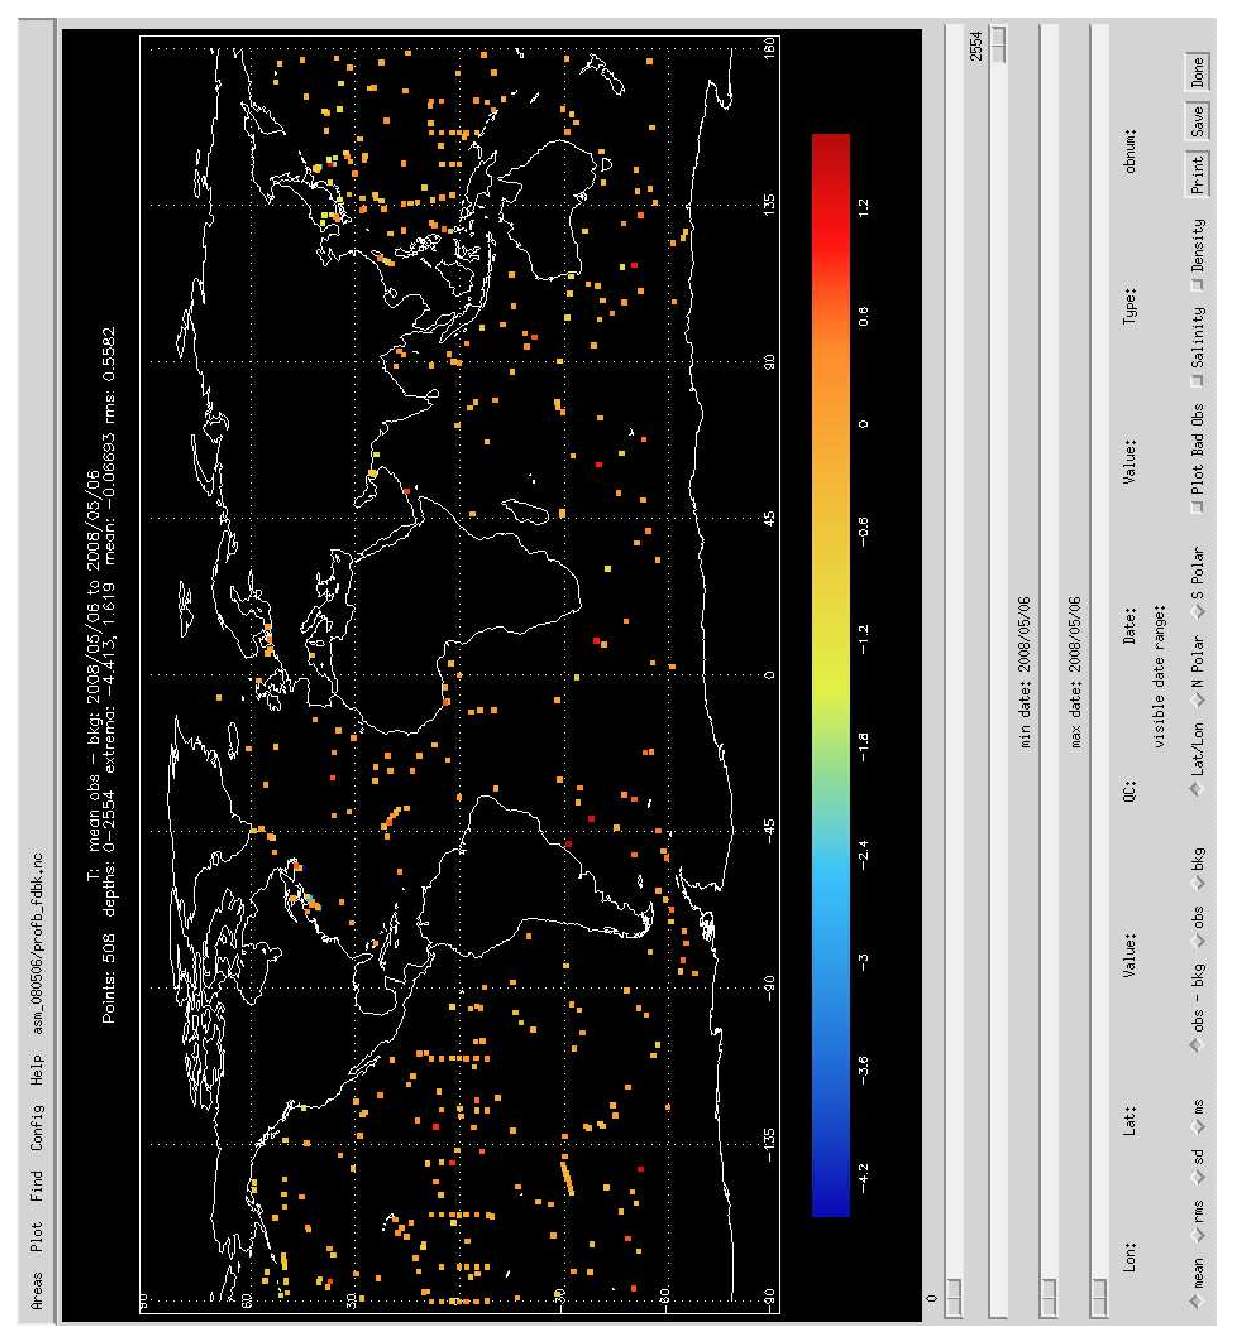
\includegraphics[width=0.66\textwidth]{OBS_dataplot_main}
  \caption{Main window of dataplot}
  \label{fig:OBS_dataplotmain}
\end{figure}

If a profile point is clicked with the mouse button a plot of the observation and background values as
a function of depth (\autoref{fig:OBS_dataplotprofile}).

\begin{figure}
  \centering
  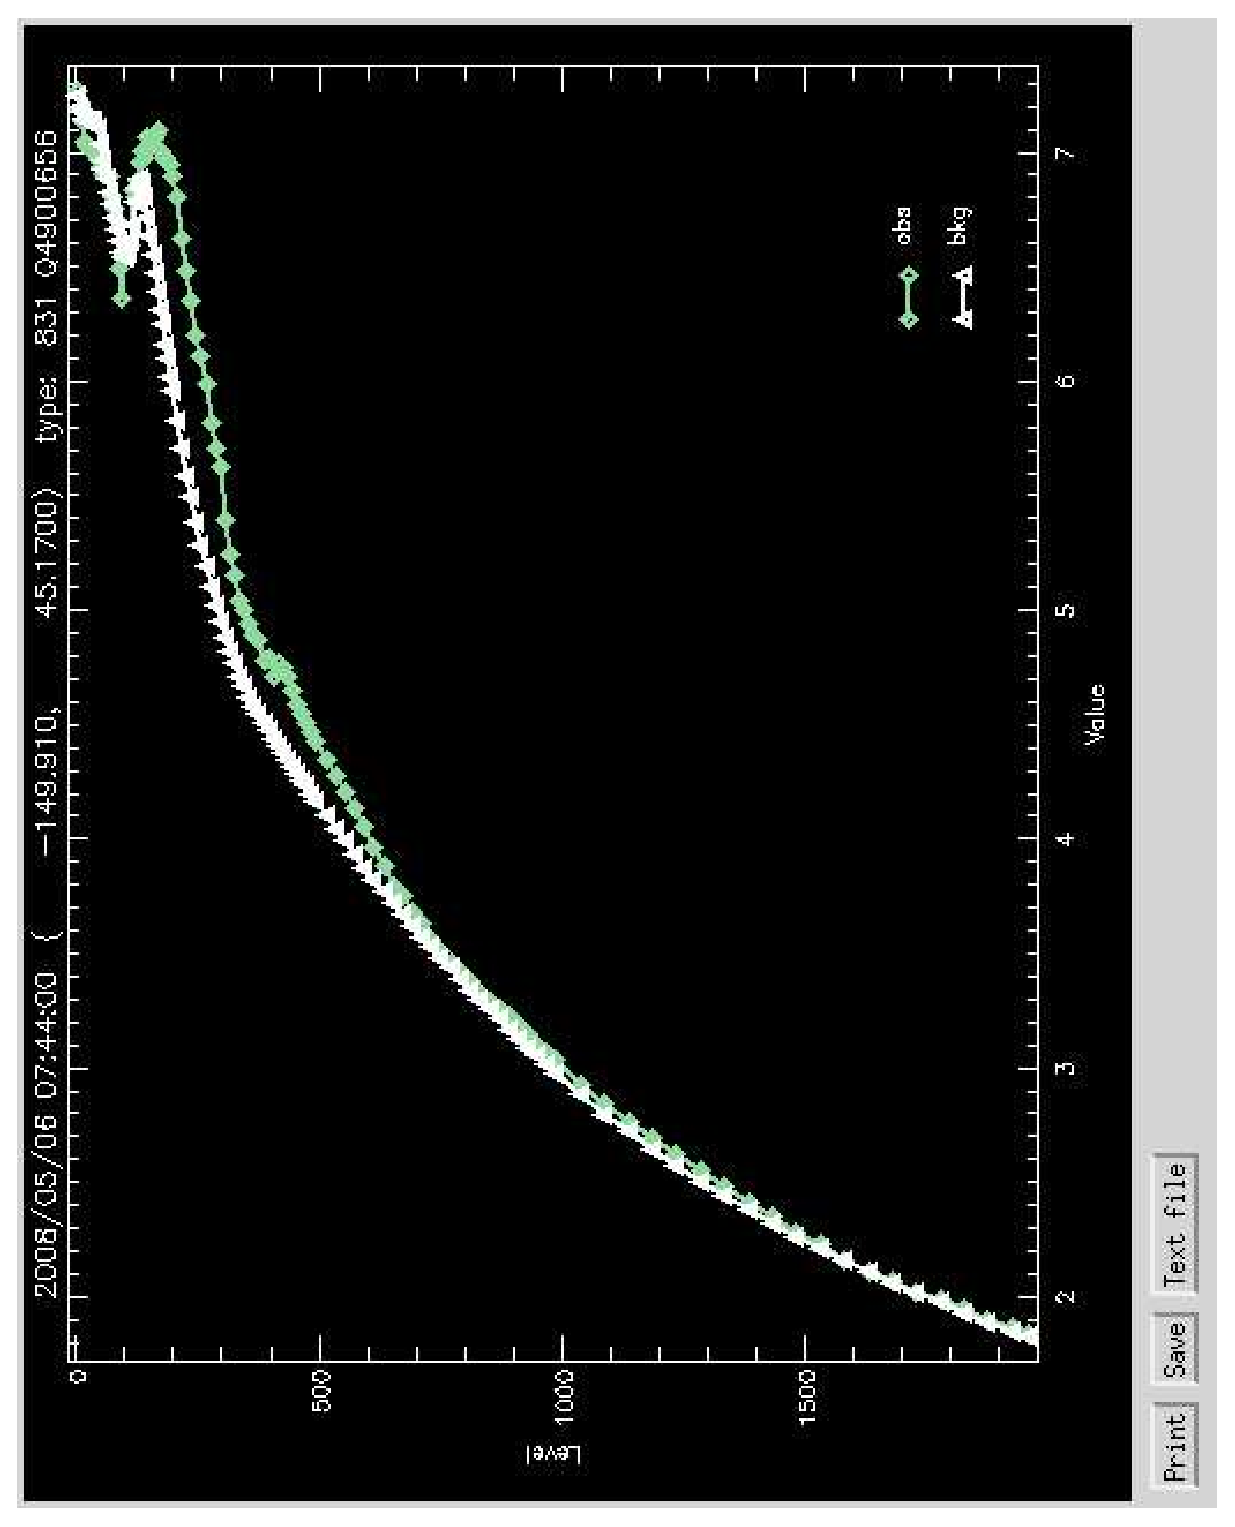
\includegraphics[width=0.66\textwidth]{OBS_dataplot_prof}
  \caption[Profile plot from dataplot]{
    Profile plot from dataplot produced by right clicking on a point in the main window}
  \label{fig:OBS_dataplotprofile}
\end{figure}

\subinc{%% =================================================================================================
%% Backmatter
%% =================================================================================================

%% Bibliography
%% =================================================================================================

\phantomsection
\addcontentsline{toc}{chapter}{Bibliography}
\lohead{Bibliography}
\rehead{Bibliography}
\bibliography{../main/bibliography}

\clearpage

%% Indices
%% =================================================================================================

\phantomsection
\addcontentsline{toc}{chapter}{Indices}
\lohead{Indices}
\rehead{Indices}
\printindex[blocks]
\printindex[keys]
\printindex[modules]
\printindex[parameters]
\printindex[subroutines]

\clearpage

%% Glossary
%% =================================================================================================

%\phantomsection
%\addcontentsline{toc}{chapter}{Glossary}
%\lohead{Glossary}\rehead{Glossary}
%\printglossaries
}

\end{document}
